%!TEX root = ../main.tex

\section{Introduction}
\label{sec:Introduction}

The term \emph{Boundary Element Method} was coined in 1977 in three publications: Banerjee and Butterfield, Brebbia and Dominguez, and Dominguez. The mathematical foundations were established by Betti in 1872 and Somigliana in 1886 for elasticity problems. Additionally, Green in 1828 and Fredholm in 1903 made foundational contributions to potential problems.

A fair question to ask is "why do we need the BEM since we already have the FEM that solves engineering problems?". The answer is that modeling with finite elements can be ineffective and laborious for certain classes of problems. So the FEM, despite the generality of its application in engineering problems, is not free of drawbacks. The most important advantages of preferring BEM over FEM are:
\begin{enumerate}
  \item The solution is mathematically expressed as a continuous mathematical formula, namely a Boundary Integral Equation (BIE). Therefore the associated numerical method, the BEM, benefits of a discretization only over the boundary $\Gamma$ of the problem domain $\Omega$, leading to a significant reduction in the number of degrees of freedom of the numerical model (see Fig.~\ref{fig:bem-fem-mesh}).

  \begin{figure}
  \begin{center}
    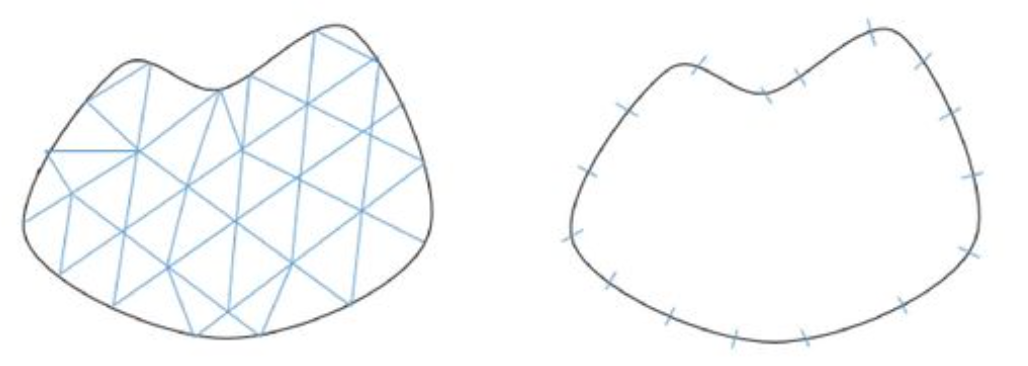
\includegraphics[width=8.4cm]{bem-fem-mesh}    % The printed column width is 8.4 cm.
    \caption{FEM versus BEM domain discretization.} 
    \label{fig:bem-fem-mesh}
  \end{center}
  \end{figure}

  \item The method is particularly effective in computing accurately the derivatives of the field function (e.g., fluxes, strain, stresses, moments).  Instead, in FE methods the accuracy drops considerably in areas of large gradients.

  However, we mention that in mixed Neumann Dirichlet problems with Lipschitz domain there arises an issue when considering continuous elements. A possible solution is the so-called double node technique, where, thanks to the splitting of a physical node into more computational nodes, continuity is preserved only on the solution, while its normal gradient is allowed to have a jump across physical edges.

  \item For infinite domains, the problem is formulated simply as an exterior one. In this manner, computer programs developed for finite domains can be used, with just a few modifications, to solve problems in infinite domains. This is not possible with the FEM.

  \item Even if nowadays there a lot of advanced professional FE softwares equipped with automatic and adaptable mesh generators, the BEM is well suited for solving problems in domains with geometric peculiarities, such as cracks and holes. Moreover, BEM is more feasible for problems described by differential equations of fourth or higher order (e.g., plate equation).
\end{enumerate}

On the other hand, the BEM exhibits the following main disadvantages:
\begin{enumerate}
\setcounter{enumi}{5}
  \item Application of the BEM requires the establishment of the BIE. This is possible only if the problem is linear and its fundamental solution can be established, such as for Laplace equation, Helmholtz equation, and Stokes system. Hence, the method cannot be used for problems whose fundamental solution is either unknown or cannot be determined. Such are, for example, problems described by differential equations with variable coefficients.

  \item The numerical implementation of the BEM results in systems of linear algebraic equations whose coefficient matrices are fully populated and nonsymmetrical. Moreover, if one considers mixed Neumann Dirichlet boundary value problems the final linear system is generally ill conditioned. In a FEM model, however, the corresponding matrices have some very nice properties, they are banded and symmetric. This drawback of the BEM is counterbalanced by a smaller dimension of its matrices (see Fig.~\ref{fig:bem-fem-grid}).

  \begin{figure}
  \begin{centering}
    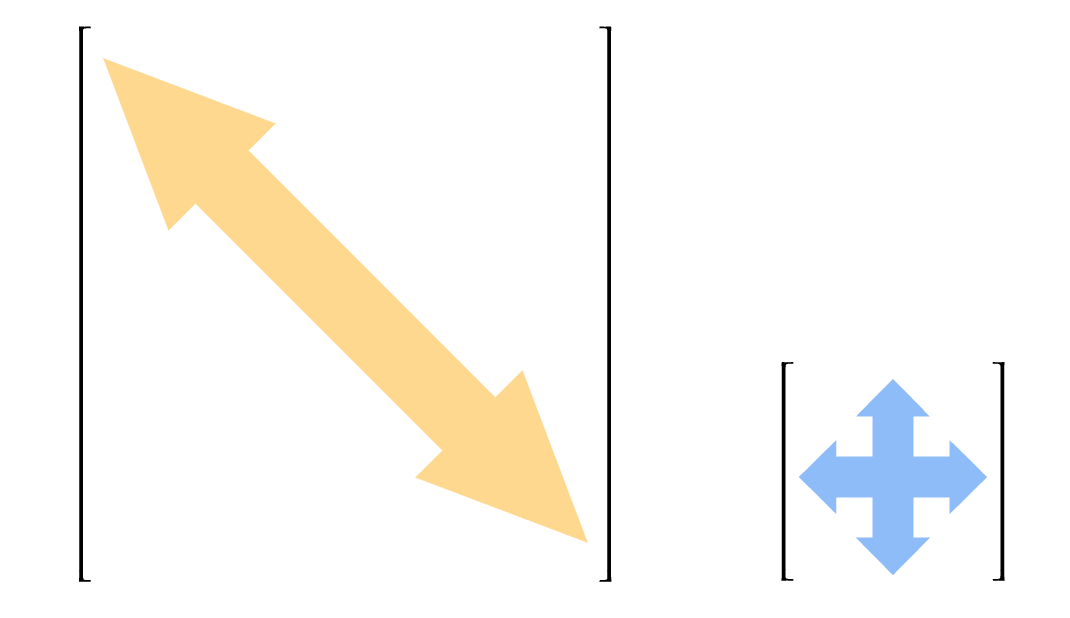
\includegraphics[width=8.4cm]{bem-fem-grid.png}
    \caption{FEM versus BEM coefficient matrix.}
    \label{fig:bem-fem-grid}
  \end{centering}
  \end{figure}
\end{enumerate}

A number of steps are possible to improve the applicability of BEM. We begin by discussing high order elements, which reduce the number of degrees of freedom needed to achieve a certain tolerance in problems with smooth solutions. High order BEMs are more attractive when compared to their FE counterparts, since increasing the order in finite elements leads to a denser, more ill conditioned system matrix. In the case of BEM the matrices, accordingly to drawback (7), are already full, and this is no more a disadvantage. If the solution is non smooth, one can combine high order elements with local refinement techniques to achieve the same result.

As the size of problem increases, none of these techniques alone is enough to reduce memory problems. Then it is usually applied a domain decomposition by exploiting distributed memory techniques, which reduce the number of degree of freedom handled by each processor. Moreover, in order to optimize BEM matrix-vector product operations from $\mathcal{O}(N^2)$ to $\mathcal{O}(N)$ it has been developed the so-called Fast Multipole Method (FMM), which thanks to a hierarcical structure (see Fig.~\ref{fig:hiera}) can decompose short and long range interaction. 

\begin{figure}
  \begin{center}
    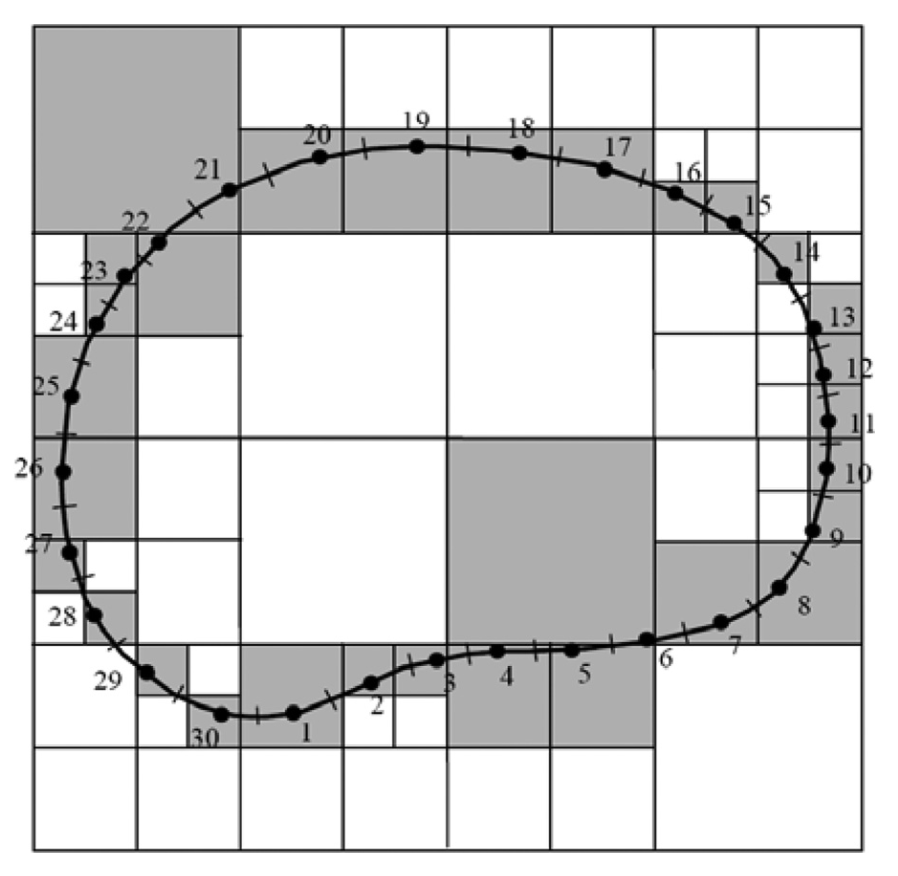
\includegraphics[width=4.2cm]{hiera1} \\
    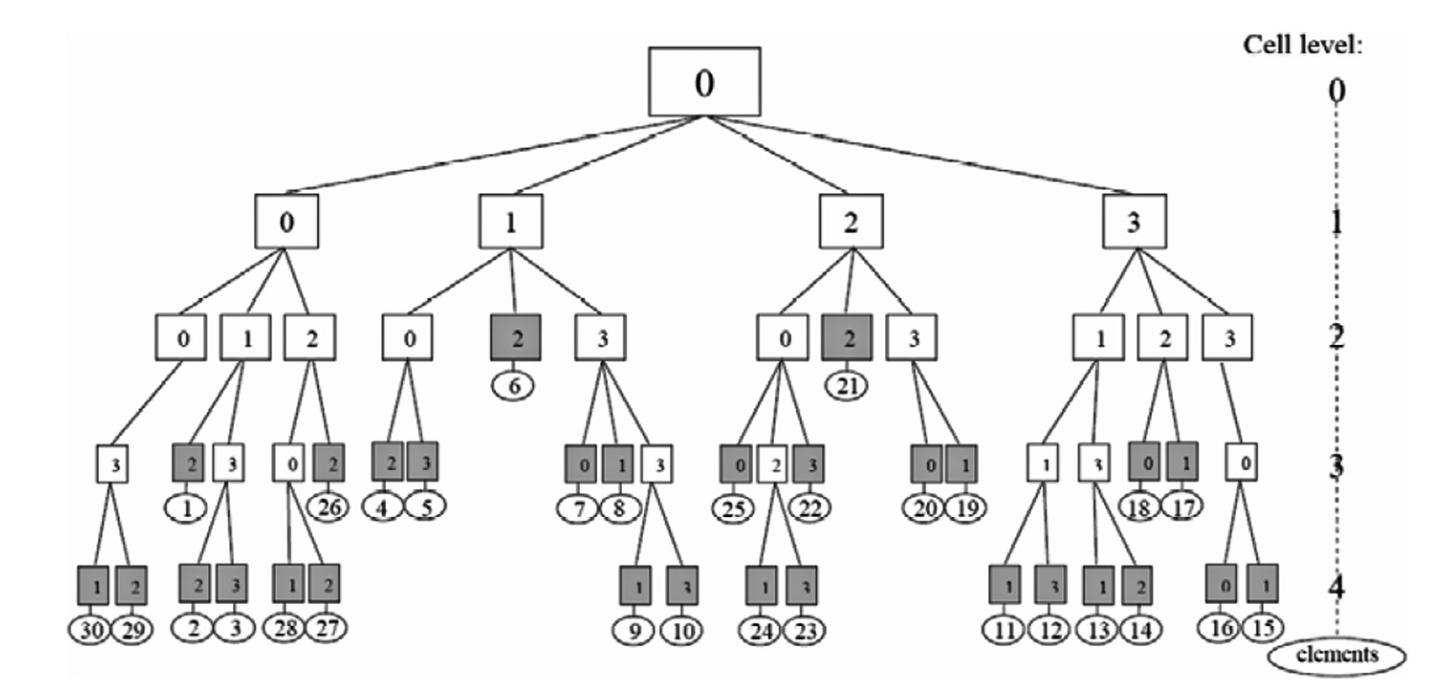
\includegraphics[width=8.4cm]{hiera2}   % The printed column width is 8.4 cm.
    \caption{Hierarchical quad-tree structure for a 2D boundary element mesh.} 
    \label{fig:hiera}
  \end{center}
\end{figure}

Nowadays, boundary integral formulation and in particular the Fast Multipole BEM (FMBEM) have been applied to problems involving hydrodynamic flows (e.g., Fig.~\ref{fig:fish}), flow around aerodynamic lifting bodies, structural mechanics, electrostatics, quantum mechanics, and acoustics (e.g., Fig.~\ref{fig:skipjack}-\ref{fig:dummy-head}). See~\ref{Katsi},\ref{Attilio} for more delailed explanations. 

\begin{figure}
  \begin{center}
    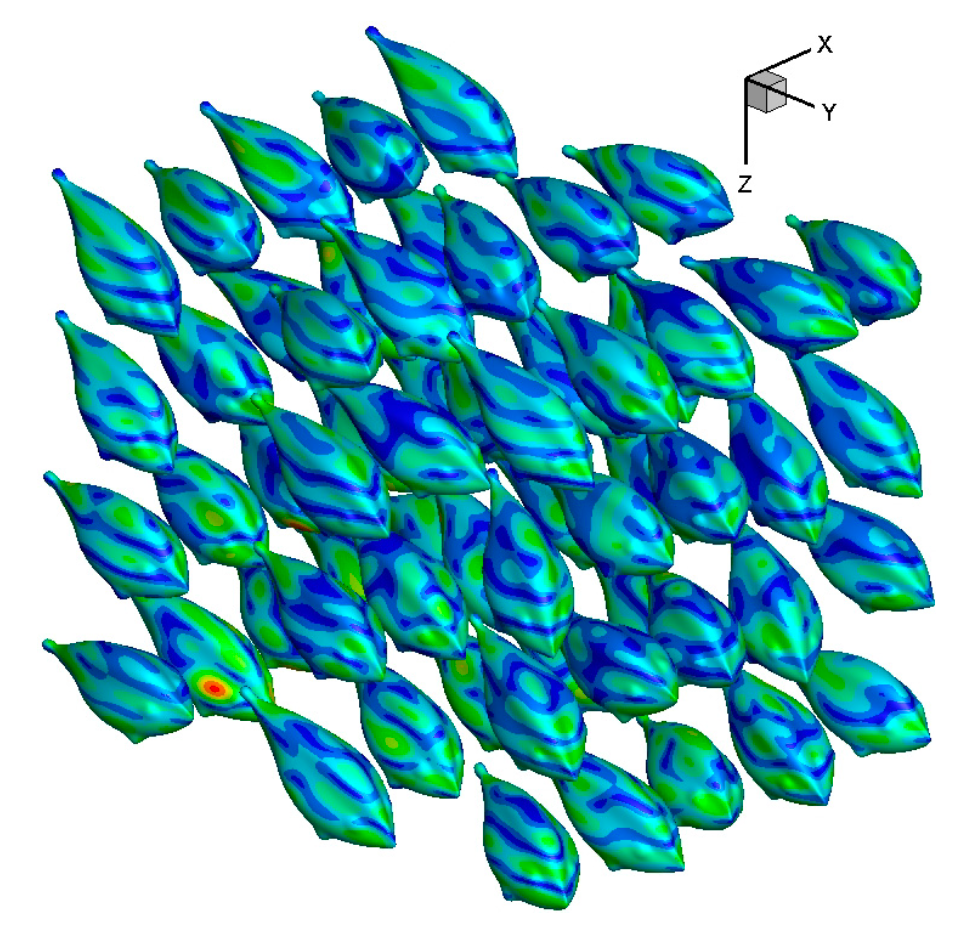
\includegraphics[width=5.6cm]{fish}    % The printed column width is 8.4 cm.
    \caption{Scattering of a multiple fish model.} 
    \label{fig:fish}
  \end{center}
\end{figure}

\begin{figure}
  \begin{center}
    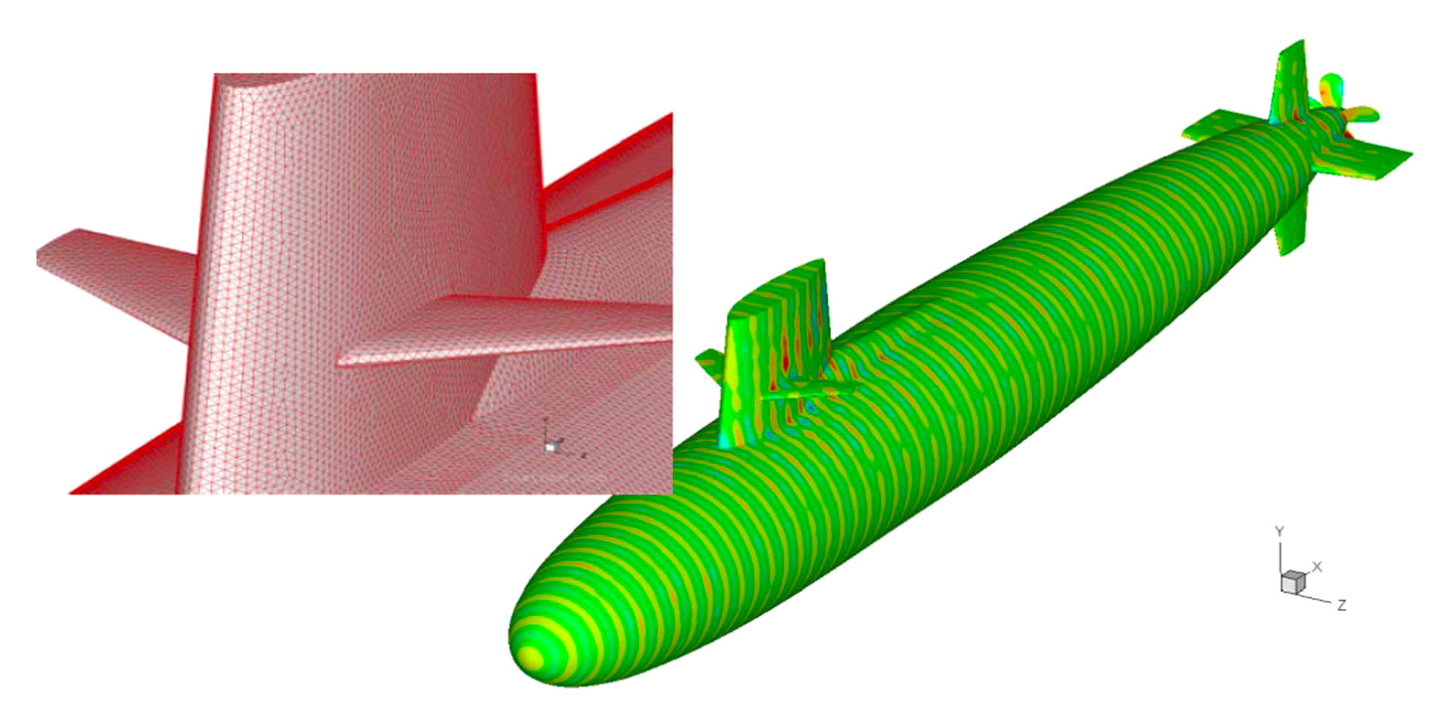
\includegraphics[width=8.4cm]{skipjack}    % The printed column width is 8.4 cm.
    \caption{BEM model of the Skipjack submarine impinged upon by an incident wave in the direction $(1, 0, \text{-}1)$.} 
    \label{fig:skipjack}
  \end{center}
\end{figure}

\begin{figure}
  \begin{center}
    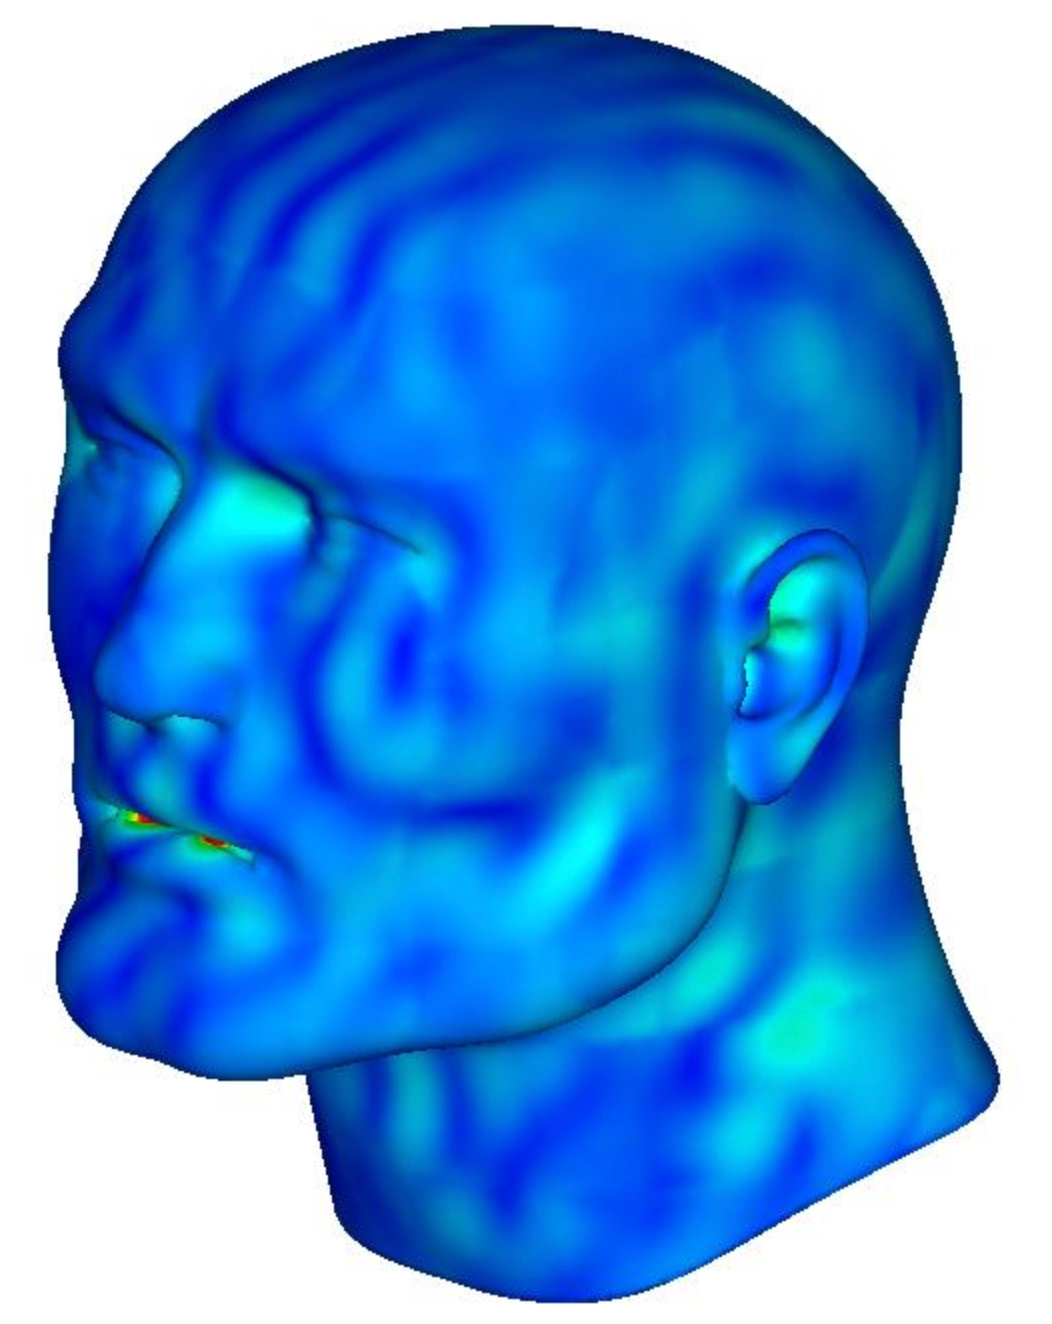
\includegraphics[width=4.2cm]{dummy-head}    % The printed column width is 8.4 cm.
    \caption{BEM mesh and sound-pressure plots for a human-head model.} 
    \label{fig:dummy-head}
  \end{center}
\end{figure}

In ths work, we are going to present for a model Laplace problem the theoretical background of BEM methodologies, as well as convergence and scalability tests of the parallel implementation carried out in \ref{Mola}.







